%%%%%%%%%%%%%%%%%%%%%%%%%%%%%%%%%%%%%%%%%%%%%%%%%%%%%%%%%%%%%%%%%%% SECTION FOUR
%%%%%%%%%%%%%%%%%%%%%%%%%%%%%%%%%%%%%%%%%%%%%%%%%%%%%%%%%%%%%%%%%%%%%%%%%%%%%%%%
\section{Ramificazioni}

Con la profonda conoscenza del significato del tempo trascorso tra noi e Blumlein,
si può ora esporre il significato dello strumento altoparlante in maniera più
dettagliata e consapevole. Per l'era
Blumlein, l'altoparlante era lo strumento futuro per un tempo presente migliore.
Il suono riprodotto, alla sua giovane età, era pura magia. Oggi sappiamo bene
quanto siamo insoddisfatti della riproduzione degli altoparlanti. Quando il
primo \emph{iPhone} è stata l'unica cosa intelligente sul pianeta è stato fantastico,
un fantastico oggetto di creazione. Oggi con lo stesso oggetto non faremmo
nemmeno una foto. Ascoltare un assolo di violino riprodotto dal miglior
altoparlante sul mercato non rappresenta la stessa esperienza della performance reale.
L'artificio non è legato alla stereofonia e all'abilità tecnica, è parte integrante del
limite della tecnologia di riproduzione che siamo in grado di realizzare.

\emph{Una voce in una piccola stanza riverberante è una condizione d'ascolto
stereofonica?} Abbiamo chiarito, con l'ausilio delle parole di Blumlein, che lo è.

\begin{quotation}
When recording music considerable trouble is experienced with the unpleasant
effects produced by echoes wich in the normal way would not be noticed by anyone
listening in the room in which the performance is taking place. [\ldots]
When the music is reproduced through
a single channel the echoes arrive from the same direction as the direct sound
so that confusion results.
\end{quotation}

Sostituendo la voce umana con la sua registrazione riprodotta da un singolo
altoparlante perdiamo, come descritto da Blumlein, la capacità del sistema
orecchie-cervello di decifrare la relazione originaria tra suono e ambiente.
Non è più lo stesso ascolto stereofonico. Diventa un altro aslcolto, una nuova
condizione di ascolto. Il numero di fonti è lo stesso. Entrambi nel loro
linguaggio monofonico producono una diversa condizione di ascolto.

Nel 1992 Michael Gerzon disegna una rappresentazione schematica delle diverse
posizioni degli altoparlanti per stereo multispeaker, da una a cinque:

\begin{quotation}
\ldots we show the loudspeaker layouts considered for frontal stage stereo
using from one (regarding mono as the trivial case of “one-loudspeaker stereo”!)
to five loudspeakers\footnote{\cite{mg92pdmsss} - mostriamo le disposizioni
degli altoparlanti considerati per lo stereo frontale partendo da uno
(considerando il mono come il banale caso dello “stereo con un solo altoparlante”!}.
\end{quotation}

Esiste una condizione di stereofonia possibile con un solo altoparlante? Ovviamente si.

Un altoparlante è in grado di suonare se stesso, il suo mondo elettrico, svincolato
dalla riproduzione di qualcosa di acustico. Un altoparlante solo, di qualsiasi tipo,
può essere messo nella condizione stereofonica di produrre un suono che non esisterebbe di esso,
con caratteristiche generali, di stereofonia e percezione binaurali assimilabili alla voce parlante.
Un rumore rosa filtrato che canta monofonicamente in una stanza è una meravigliosa condizione di stereofonia.

\subsection{Sullo strumento \emph{Altoparlante}}

L'enciclopedia britannica cataloga con una inequivocabile descrizione il termine
\emph{Loudspeaker: SOUND INSTRUMENT}. Il passaggio da altoparlante, strumento
sonoro, ad altoparlante strumento musicale, è breve, è necessario solo un musicista.

La scelta dell'altoparlante, la conoscenza del suo carattere e delle caratteristiche
tecniche è un momento necessario per quel musicista, un momento che richiede tempo.
Cambiare manualmente la frequenza di un suono sinusoidale riprodotto da un
altoparlante a tre vie, a un metro di distanza, con le orecchie alla stessa
altezza del baricentro dello strumento, è un buon modo per conoscere l'altoparlante. Il musicista scoprirà in questo modo che i
suoni prodotti dall'altoparlante cambieranno forma durante il glissato. Forse
vicino al punto di incrocio del crossover troverà alcune peculiarità, altre
strane decorrelazioni di fase ad altissima frequenza.

Scoprire e conoscoere lo strumento altoparlante e conoscere il sistema percettivo
in termini di meccanismi psico-acustici sono condizioni necessarie per
affrontare correttamente un percorso di emancipazione nei confronti dei limiti
tecnici e tecnologici nella riproduzione, produzione elettroacustica dei suoni.
Michael Gerzon, dagli anni settanta agli anni novanta, ha descritto molteplici
approcci di risoluzione dei problemi legati alla stereofonia, sempre attingendo
alle radici dell'era Blumlein, con tentativi di progettare tecnologie di
riproduzione con lo scopo di colmare il divario rispetto al regno acustico.

\begin{quotation}
The ears and brain localize sounds according to many different mechanisms. Among
the most important cues used are low-frequency interaural phase (applicable up
to around $2KHz$, but dominant below $700Hz$) and localization by
amplitude differences between the two ears, predominantly above about
$1KHz$. While other cues are also important, we have found that satisfying
both these cues, and making them mutually consistent for central listener facing
in any direction, leads to particularly robust and reliable localization
quality.\footnote{\cite{mg92pdmsss} - Le orecchie e il cervello localizzano i
suoni secondo molti meccanismi diversi. Tra i segnali più importanti utilizzati
vi sono la fase interaurale a bassa frequenza (applicabile fino a circa $2KHz$,
ma dominante al di sotto di $700Hz$) e la localizzazione mediante
differenze di ampiezza tra le due orecchie, prevalentemente al di sopra di
circa $1KHz$. Sebbene anche altri segnali siano importanti, abbiamo
scoperto che soddisfare entrambi questi segnali e renderli reciprocamente
coerenti per l'ascoltatore centrale rivolto verso qualsiasi direzione, porta
a una qualità di localizzazione particolarmente solida e affidabile.}
\end{quotation}

%%%%%%%%%%%%%%%%%%%%%%%%%%%%%%%%%%%%%%%%%%%%%%%%%%%%%%%%%%%%%%%%%%%% SUBSECTION
%%%%%%%%%%%%%%%%%%%%%%%%%%%%%%%%%%%%%%%%%%%%%%%%%%%%%%%%%%%%%%%%%%%%%%%%%%%%%%%%
\subsection{Sul concetto di \emph{PanPot}}
\label{sec:panpot}

L'oggetto \emph{panner} è rappresentato da un potenziometro di controllo
(hardware o software, in entrambi i casi a controllo analogico o digitale) che
regola la distribuzione di un segnale su più canali componenti un campo sonoro
stereo o multicanale. Ogni mixer ha un \emph{panpot} (abbreviazione di
\emph{potenziometro di panoramica}), per ciascun canale sorgente in ingresso,
che regola l'azione del \emph{panner}.

%L'ultima precisazione riguarda il movimento panoramico. La distribuzione dell'energia
%o la condizione della coppia di segnali che regola il movimento panoramico troppo
%spesso sono descritti come la possibilità di muovere gli oggetti attorno alla posizione
%dell'ascoltatore.

Generalmente il \emph{panpot} viene descritto come un pomello che permette di
muovere i suoni tra la sinistra e la destra del panorama di diffusione, il che è
parzialmente vero e potenzialmente pericoloso in termini di immaginazione
acustica.

Soffermandosi ad analizzare il fenomeno acustico di un suono prodotto da un
oggetto in movimento tra la destra e la sinistra di un campo percettivo emergono
diversi problemi.

Il primo riguarda l'\emph{effetto doppler}. Siamo seduti su una panchina al
margine di una strada che si estende infinita agli estremi della nostra vista
periferica. Un mezzo di soccorso, con la sirena accesa, si avvicina percorrendo
la strada davanti al nostro viso, da sinistra verso destra: percepiamo
una variazione in frequenza al passaggio della sirena, in funzione della
velocità. L'\emph{effetto doppler} ci descrive come nel percorso di
avvicinamento a noi la frequenza sale lentamente fino al massimo ottenuto nel
momento in cui ci raggiunge per poi diminuire rapidamente in coincidenza con
l'allontanamento.

Ora siamo dei \emph{sound designer}, siamo seduti di fronte alla nostra console
analogica e dobbiamo replicare l'effetto sopra descritto. Applicando un
movimento da sinistra a destra, azionando il \emph{panpot} su un suono di sirena
statico, registrato fermo ad un metro di distanza, pur ruotando velocemente il
potenziometro non otteniamo variazioni in frequenza. Il suono si muove tra la
sinistra e la destra del sistema d'ascolto senza produrre il movimento nello
spazio ma solamente lo spostamento della posizione relativa al nostro punto di
ascolto. Ne deriva una prima conslusione: il \emph{panpot} regola una posizione
relativa, non stabilisce criteri di movimento.

Un altro problema emergente del pensare il \emph{panning} come un movimento
scaturisce dalla relazione della sorgente con l'ambiente circostante. Che
movimento può esserci senza tenere conto del luogo in cui la sorgente sonora si
trova? Un avvocato pronuncia la sua arringa in tribunale parlando ad alta voce,
camminando, rimbalzando tra destra e sinistra. La voce si propaga nello spazio
ed è inevitabile che se ne percepisca la variazione topologica, morfologica in
relazione con le caratteristiche architettoniche: a sinistra della stanza c'è
una parete di finestre, a destra un muro in cemento. Pur non avendo velocità
sufficiente ad innescare l'effetto doppler, la sua continua variazione di
posizione corrisponde ad una continua variazione di rapporto con l'ambiente che
lo circonda, in relazione ad ogni infinto punto di ascolto all'interno della
stanza. In altre parole, quel movimento assume significati diversi relativi al
punto di ascolto.

Dovendo simulare lo stesso effetto mediante l'azione sul panpot, otterremmo la
variazione di posizione della voce nello spazio, ma non la sua relazione con lo
spazio.

\begin{figure*}[t!]
    \centering
    \begin{subfigure}[t]{0.45\textwidth}
        \centering
        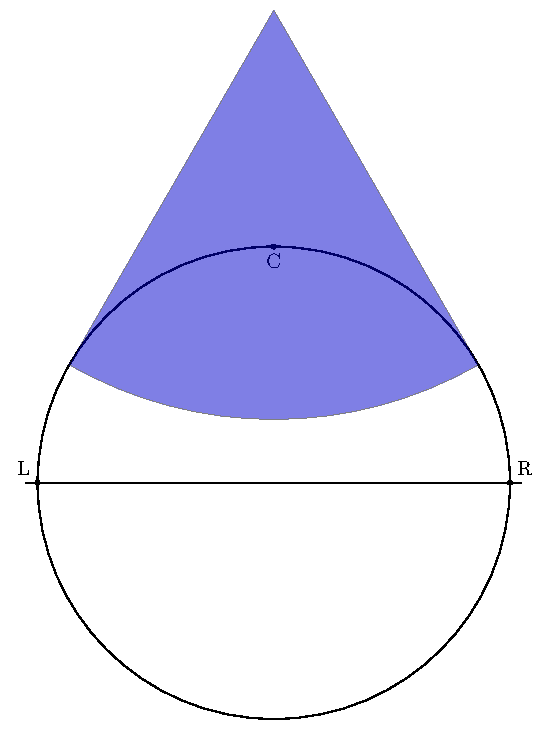
\includegraphics[height=8cm]{CAPITOLI/_TIKZ/PANNING/pan-frontal}
        \caption{Sorgente con incidenza frontale.}
        \label{pan:frontal}
    \end{subfigure}%
    ~
    \begin{subfigure}[t]{0.45\textwidth}
        \centering
        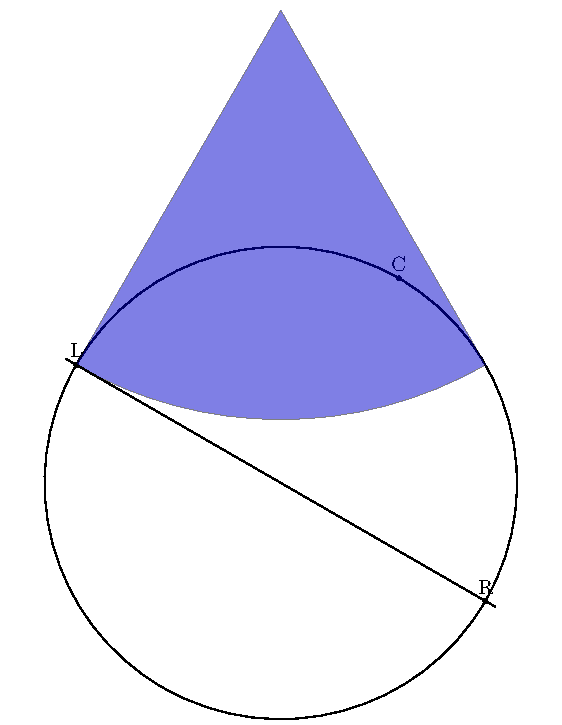
\includegraphics[height=8cm]{CAPITOLI/_TIKZ/PANNING/pan-left}
        \caption{Sorgente con incidenza laterale sinistra di 30 gradi.}
        \label{pan:left}
    \end{subfigure}
    \\
    \begin{subfigure}[t]{0.9\textwidth}
        \centering
        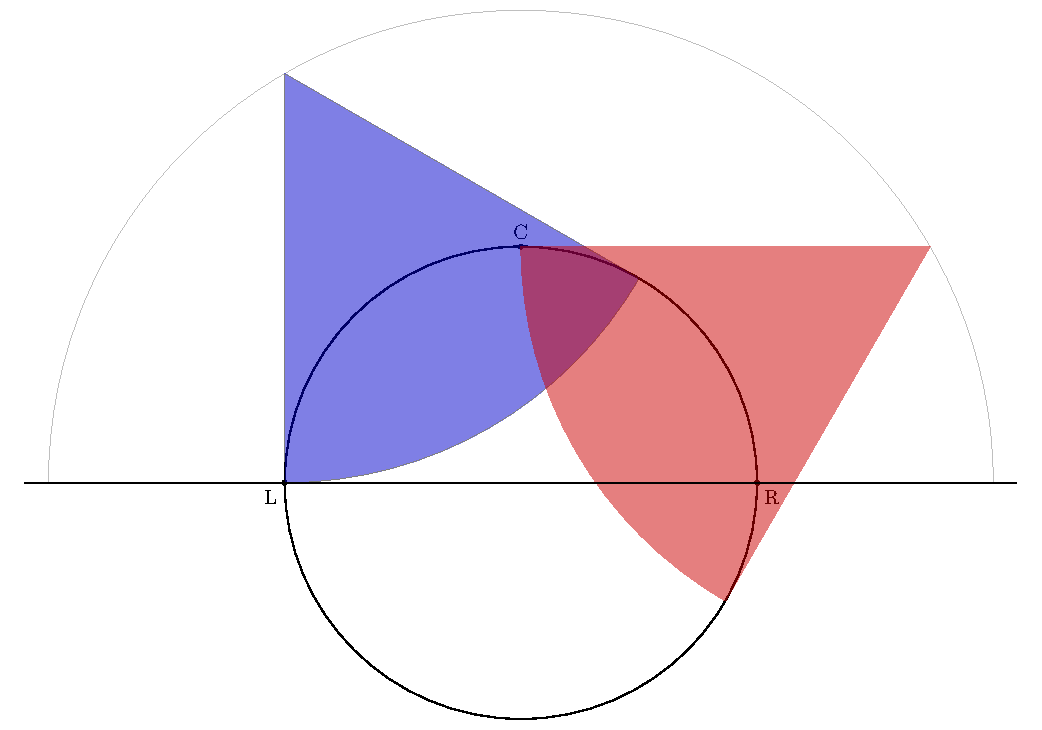
\includegraphics[height=8cm]{CAPITOLI/_TIKZ/PANNING/pan-both}
        \caption{Due sorgenti, una con incidenza laterale sinistra di 30 gradi,
        l'altra con incidenza laterale destra di 60 gradi.}
        \label{pan:both}
    \end{subfigure}
    \caption{La rotazione del \emph{PanPot} esegue una modifica della condizione
    di ascolto dell'ascoltatore, non un movimento della sorgente. Posizionando
    le singole sorgenti ci si pone in ascolto laterale, ruotati. Nella
    sovrapposizione di molteplici sorgenti il panorama risulta composto da
    ognuna di queste, con posizioni assolute ed angoli di incidenza relativi
    della testa.}
    \label{pan:all}
\end{figure*}

Il \emph{panpot}, nella sua capacità di descrizione della relazione tra i canali
che ricevono i suoi segnali, non muove la sorgente nello spazio, ma regola la
posizione della sorgente stessa in relazione al nostro punto di ascolto. In
altri termini il \emph{panner} non regola il movimento della sorgente, ma la
rotazione della testa in relazione ad essa. Il \emph{panner}, muove langolo di
incidenza del suono, ruota la testa, nei confronti della sorgente immobile.

Ogni \emph{panner} ha un'architettura interna che determina la quantità e la
condizione del segnale sorgente per ogni canale di destinazione. I più semplici
suddividono i segnali audio nei due canali sinistro e destro, attraverso un
opportuno controllo di guadagno (volume) discreto. La distribuzione dell'energia
tra i due canali è chiamata legge ed è descrivibile con una funzione matematica.

Come descritto da Blumlein, la sola variazione di ampiezza nella
rappresentazione del panorama stereofonico rappresenta una parte nella complessa
soddisfazione della percezione binaurale, non disegna l'intero meccanismo.
Per questo motivo, prima di descrivere i sistemi di panning di ampiezza, che
sono universalmente implementati su tutti i mixer del pianeta, è più opportuno
riprendere da dove egli stesso è partito. La visione di Blumlein fu ripresa in
seguito da Michael Gerzon, negli anni settanta, per sviluppare la tecnologia
\emph{ambisonic}, la quale rimane un atto di descrizione del mondo sonoro
percepito e riprodotto, nell'evoluzione della stereofonia, completamente diverso
da quello che commercialmente si è diffuso ed imposto.

%%%%%%%%%%%%%%%%%%%%%%%%%%%%%%%%%%%%%%%%%%%%%%%%%%%%%%%%%%%%%%%%%%%% SUBSECTION
%%%%%%%%%%%%%%%%%%%%%%%%%%%%%%%%%%%%%%%%%%%%%%%%%%%%%%%%%%%%%%%%%%%%%%%%%%%%%%%%
\subsection{Sul concetto di \emph{Diagramma Polare}}
\label{sec:polarplot}

La figura polare di un microfono è la rappresentazione grafica su di un piano,
nel sistema di coordinate polari, della sensibilità in funzione dell'angolo di
incidenza del suono sulla membrana. Questo tipo di figura polare si presenta
come una linea curva chiusa (o insieme di più linee di questo tipo, tipicamente
associate alle ampiezze polari in risposta a diverse frequenze). In presenza di
un’unica curva, si intende che questa è riferita ad una frequenza di $1KHz$ che
rappresenta la curva di livello relativa ad un generico valore di intensità di
risposta del microfono stesso, e come tale fornisce una rapida indicazione
visiva di come l'intensità di risposta sia geometricamente distribuita intorno
al microfono stesso.

\begin{figure}[t]
\centering
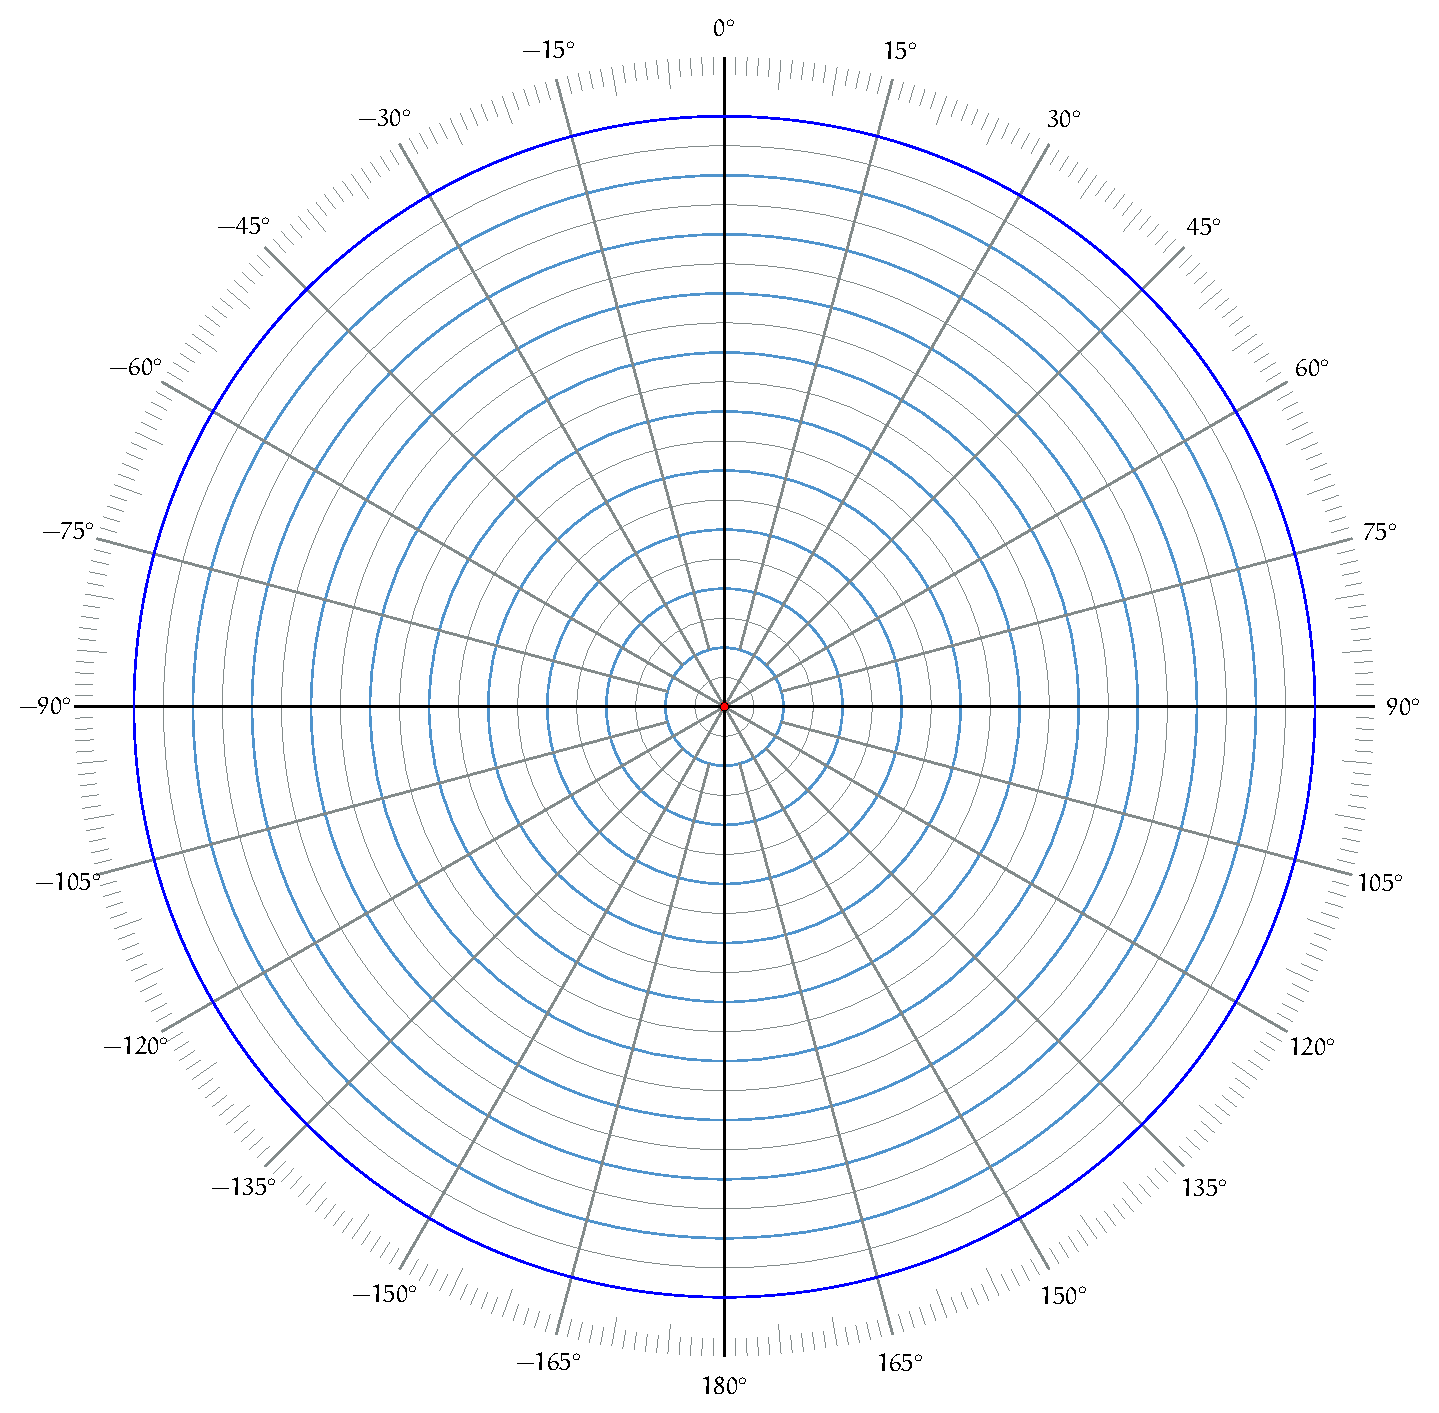
\includegraphics[width=1\columnwidth]{CAPITOLI/_TIKZ/POLAR/omni}
\caption{non-directional. Equazione: $ndp = 1(x)$}
\label{polar:omni}
\end{figure}

In un sistema polare ciascun punto è
determinato da una distanza, da un punto di riferimento, ed un angolo, da una
direzione di riferimento. Nel caso di una figura polare di un microfono, il
punto di riferimento è l'originne, il centro del piano e la direzione di
riferimento è il fronte, ovvero l'asse di puntamento frontale del microfono. Per
questa ragione la figura polare del microfonico presenta l'angolo zero
nel nord del piano, si muove angolarmente verso sinistra per angoli
negativi e verso destra per angoli positivi. Il movimento angolare, denominato
\emph{azimuth} è espresso in radianti

\begin{equation}
\theta = -\pi,\pi
\label{eq:rad}
\end{equation}

Una eventuale indicazione in gradi può essere espressa mediante l'equazione:

\begin{equation}
deg = \pi/180
\label{eq:deg2rad}
\end{equation}

Un segnale nella sua oscillazione espressa nella variazione di ampiezza
attorno allo zero potrebbe essere derivato da qualsiasi tipo di microfono senza
un significato particolare. Potrebbe essere generato elettricamente da un
microfono con modello polare particolare o generato sinteticamente secondo equazioni polari, senza
alcuna rilevanza specifica in termini di descrizione dell'andamento di ampiezza.
La provenienza polare, la forma che assume la fase del segnale, diventa rilevante nel confronto tra segnali.

Il diagramma polare di un microfono che, per caratteristiche costruttive, non
percepisce variazioni di angolo di incidenza del segnale, quindi non-direzionale,
è definito comunemente omni-direzionale, la sua equazione contiene solo
variazioni di ampiezza, derivate della variazione di pressione dell'aria
(per questo sono definiti microfoni a pressione)

\begin{equation}
ndp = 1(x)
\label{eq:omni}
\end{equation}

%Il disegno nella parte sinistra di fig. 8 rappresenta la struttura di un tipico microfono a pressione (pressure microphone) omnidirezionale, mentre nella parte destra è rappresentata la sua curva polare, dove vediamo che la direzionalità del suono inizia ad essere percepita dal microfono a partire da circa 5 KHz in su, mentre le frequenze gravi non sono indicate in quanto assimilabili a quella rilevata a 1 KHz, cioè con attenuazione zero per qualsiasi angolo di provenienza del suono.

I microfoni che hanno caratteristiche di direzionalità vengono definiti a
gradiente di pressione in quanto la variazione di pressine dell'aria è percepita
in maniera diversa per angoli d'incidenza diversi. Tra questi il microfono bidirezionale,
dennominato a \emph{figura-8}, presenta una simmetria fronte/retro, dove i punti di
attenuazione massima si vanno a situare a $\pm90°$. Tali microfoni hanno uguale
sensibilità per i suoni provenienti dal fronte e dal retro, mentre tendono ad
annullare i suoni di provenienza laterale.

\begin{equation}
bpg = x\cos\theta
\label{eq:fig8}
\end{equation}

\begin{figure}[t]
\centering
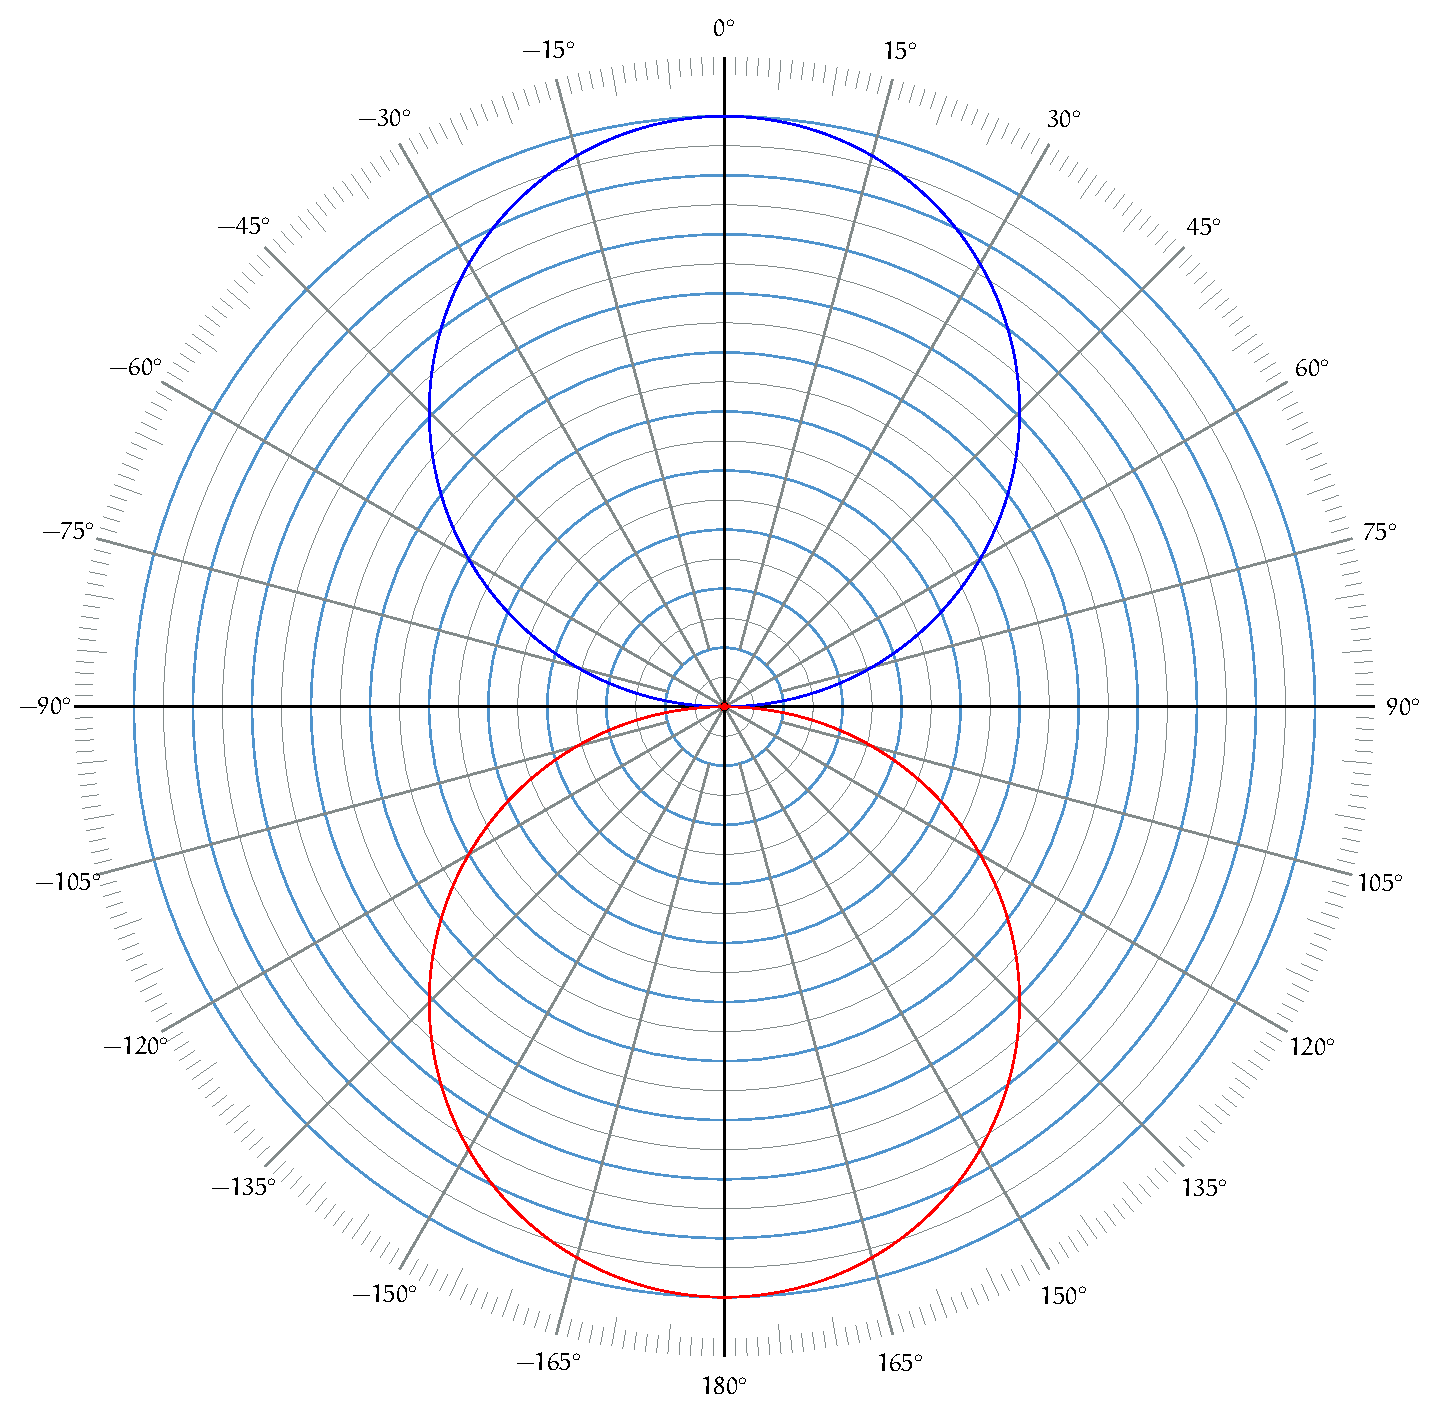
\includegraphics[width=1\columnwidth]{CAPITOLI/_TIKZ/POLAR/fig8}
\caption{Figure-8}
\label{polar:fig8}
\end{figure}

La prima differenza rilevante tra un'equazione del modello polare non
direzionale (\ref{eq:omni}) e una direzionale (\ref{eq:fig8}) è la
presenza del coefficiente angolare. L'angolo \emph{theta} nell'equazione
(\ref{eq:fig8}) descrive la direzione di puntamento del microfono bidirezionale
espressa in radianti. $x$ è il segnale relativo alla pressione.

Il microfono cardioide (\emph{cpg}) che tentiamo di sintetizzare deve puntare
alla posizione centrale-anteriore che è il riferimento zero radianti.

Il microfono cardioide del primo ordine potrebbe essere descritto come una somma delle
variazioni di pressione non direzionale (\emph{ndp})


\begin{equation}
cpg = 0.5(x) + 0.5(x\cos\theta)
\label{eq:cardioid}
\end{equation}

\begin{figure}[t]
\centering
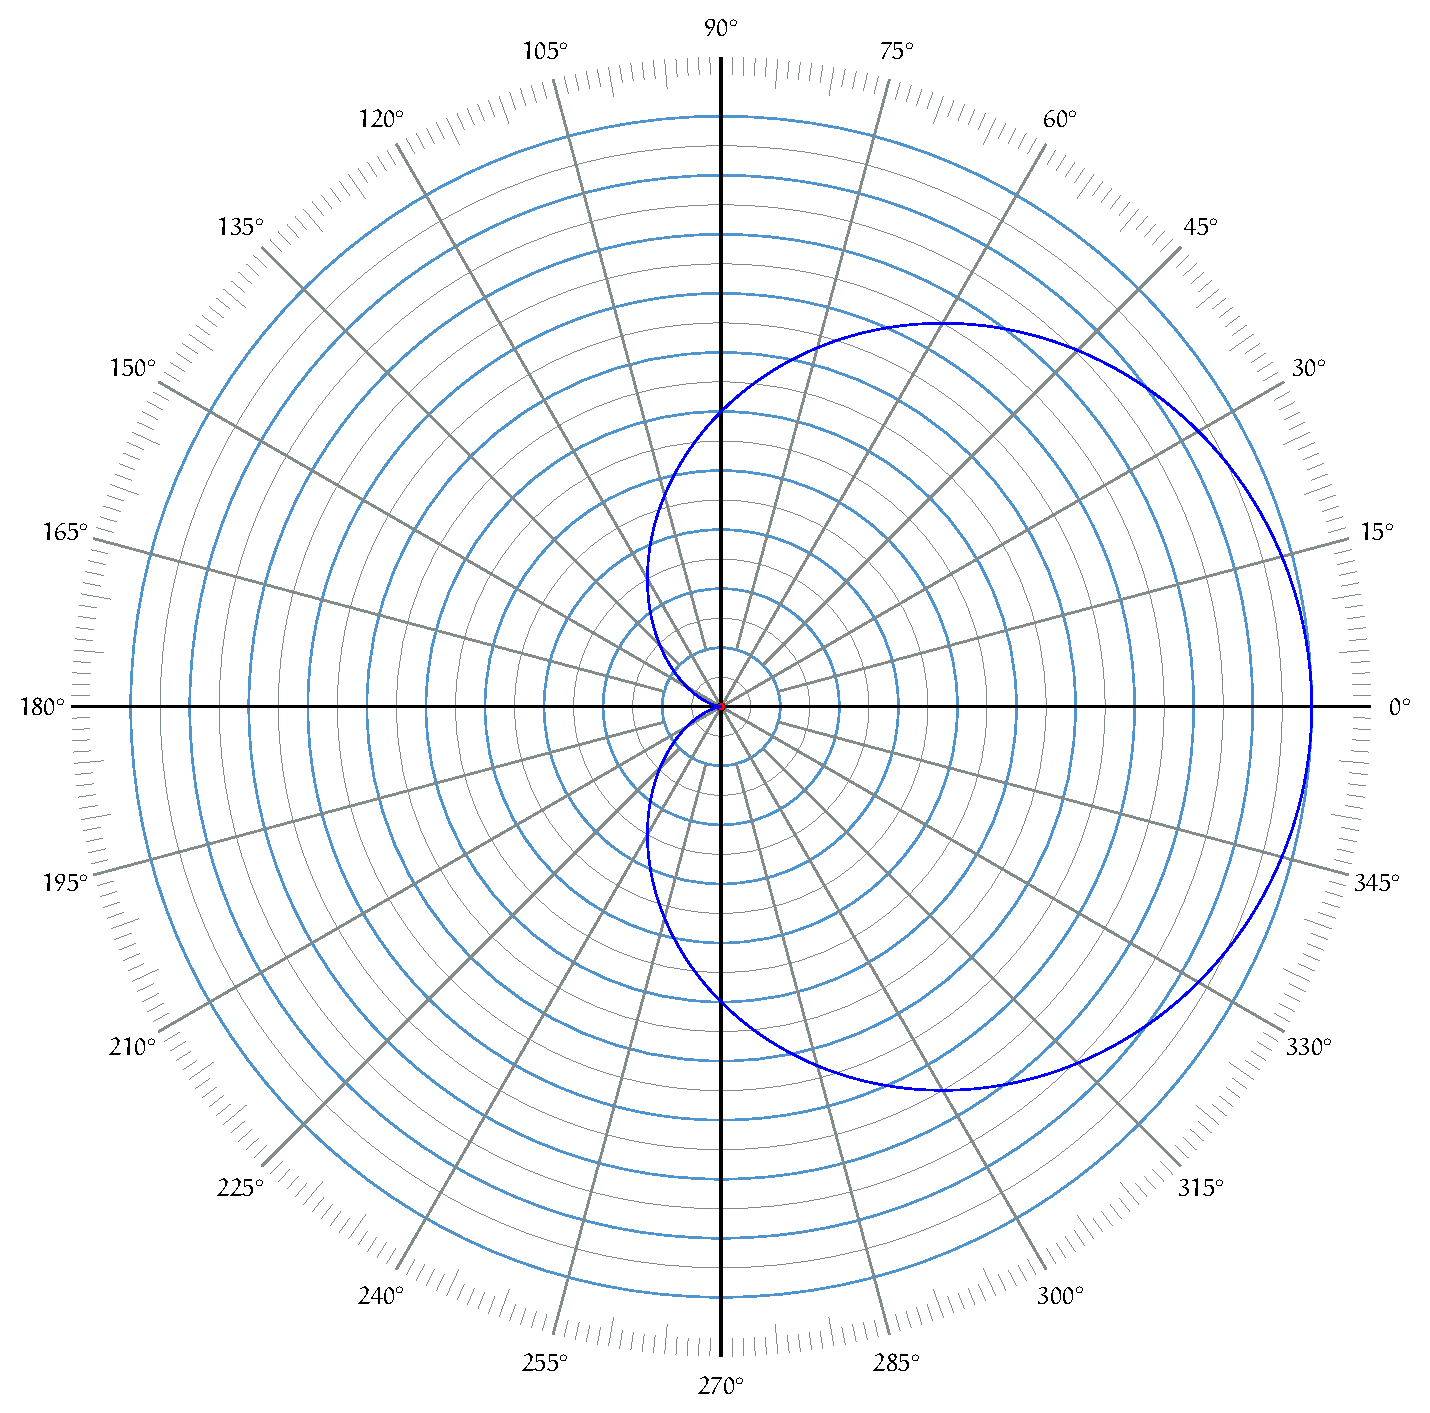
\includegraphics[width=1\columnwidth]{CAPITOLI/_TIKZ/POLAR/cardioid}
\caption{Cardioid}
\label{polar:cardioid}
\end{figure}

Cardioidi e altri schemi più comuni del primo ordine sono prodotti con il
diversi coefficienti di peso tra la pressione non-direzionale e gradiente di pressione
bidirezionale, come in tabella \ref{tab:polarcoef}.

\begin{table}[ht]
\begin{center}
\begin{tabular}{cc}
\textbf{Polar Pattern} & \textbf{Equation} \\
\hline
non-direzionale & $1(x)$ \\
subcardioide    & $0.75(x)+0.25(x\cos\theta)$ \\
cardioide       & $0.5(x)+0.5(x\cos\theta)$ \\
supercardioide  & $0.37(x)+0.63(x\cos\theta)$ \\
ipercardioide   & $0.25(x)+0.75(x\cos\theta)$ \\
bidirezionale   & $1(x\cos\theta)$ \\
\end{tabular}
\end{center}
\caption{Coefficienti di pressione \emph{non-direzionale} e gradiente di pressione
\emph{bidirezionale} per la descrizione dei modelli polari intermedi, del primo ordine.
Dove $x$ è la variazione d'ampiezza del segnale, e $\theta$ l'angolo di incidenza}
\label{tab:polarcoef}
\end{table}

Quindi dai primitivi schemi polari del primo ordine, non direzionali e
bidirezionali, potremmo derivare, progressivamente, ogni sfumatura di forma tra
di loro, puntando angolarmente ovunque intorno a $2\pi$ radianti.

\begin{figure*}[h]
    \centering
    \begin{subfigure}[t]{0.3\textwidth}
        \centering
        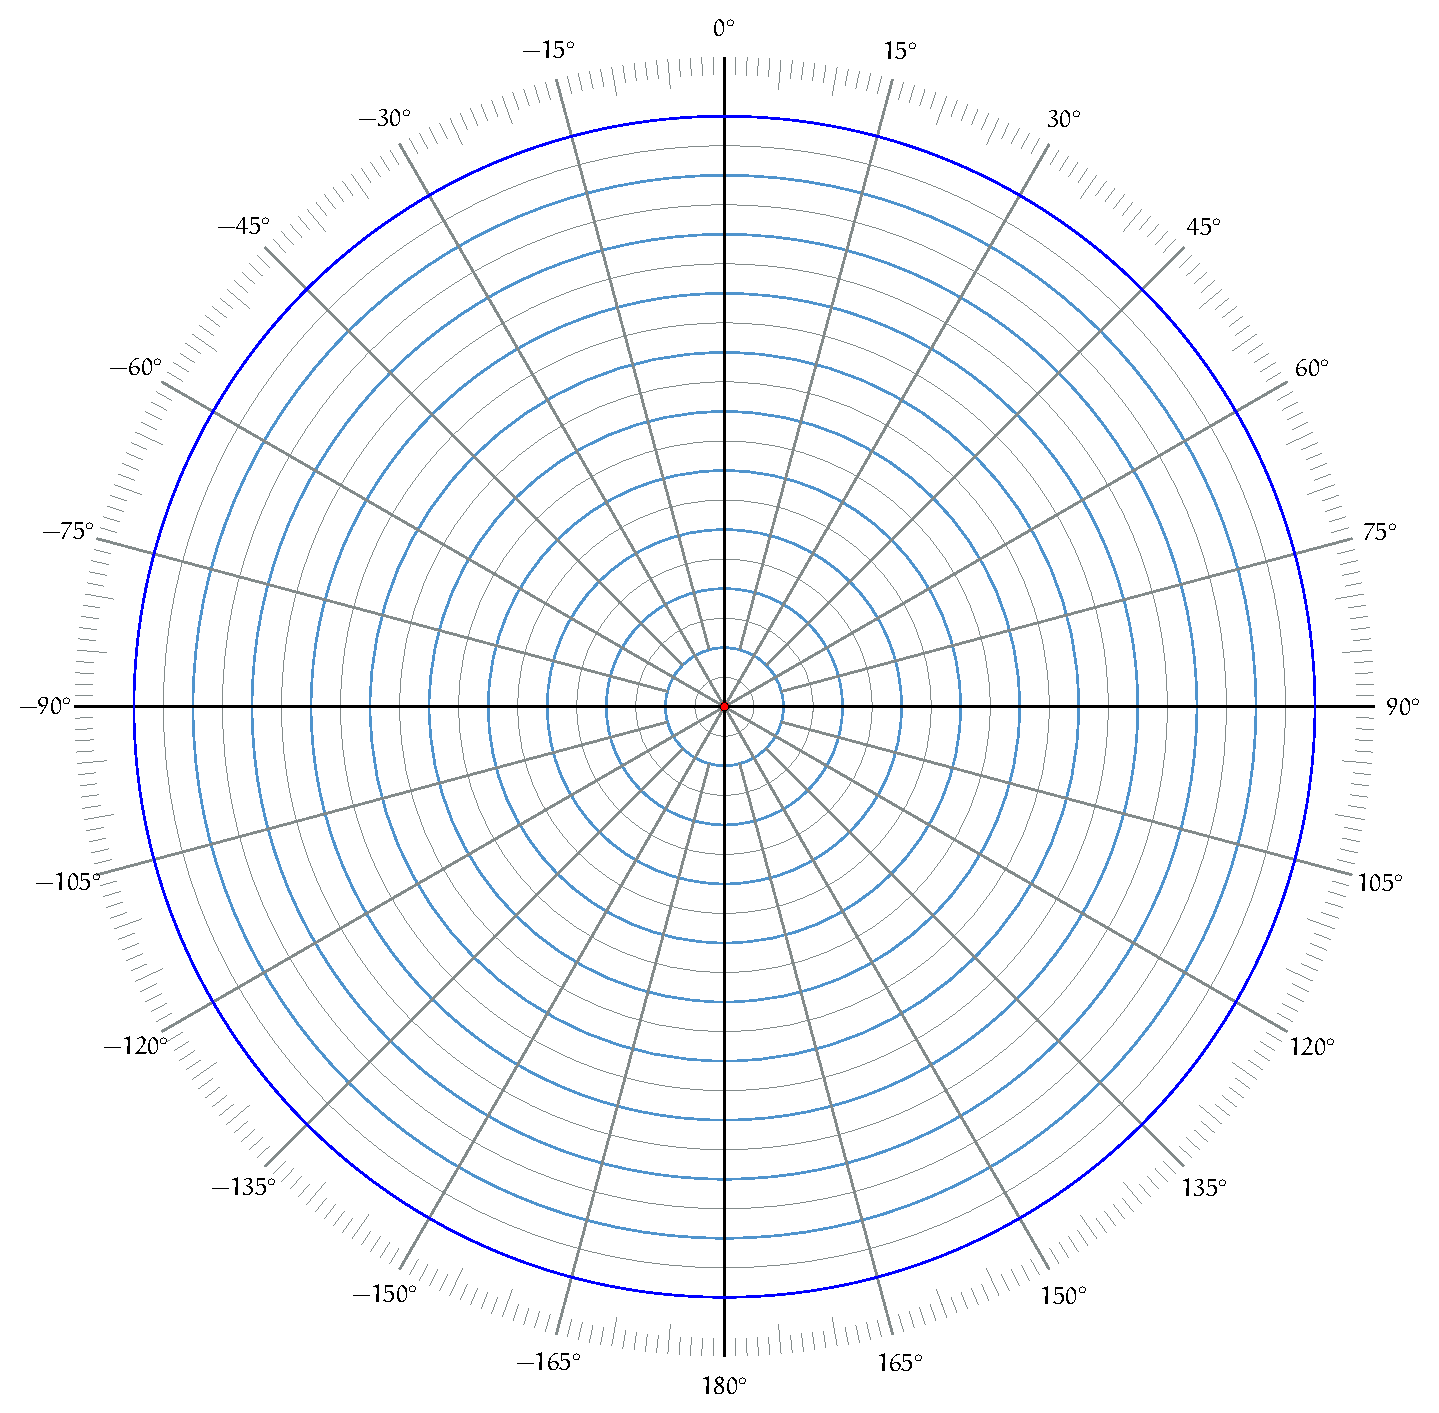
\includegraphics[height=4cm]{CAPITOLI/_TIKZ/POLAR/omni}
        \caption{non-direzionale. \\ Eq: $1(x)$}
        \label{pol:omni-p}
    \end{subfigure}%
    ~
    \begin{subfigure}[t]{0.3\textwidth}
        \centering
        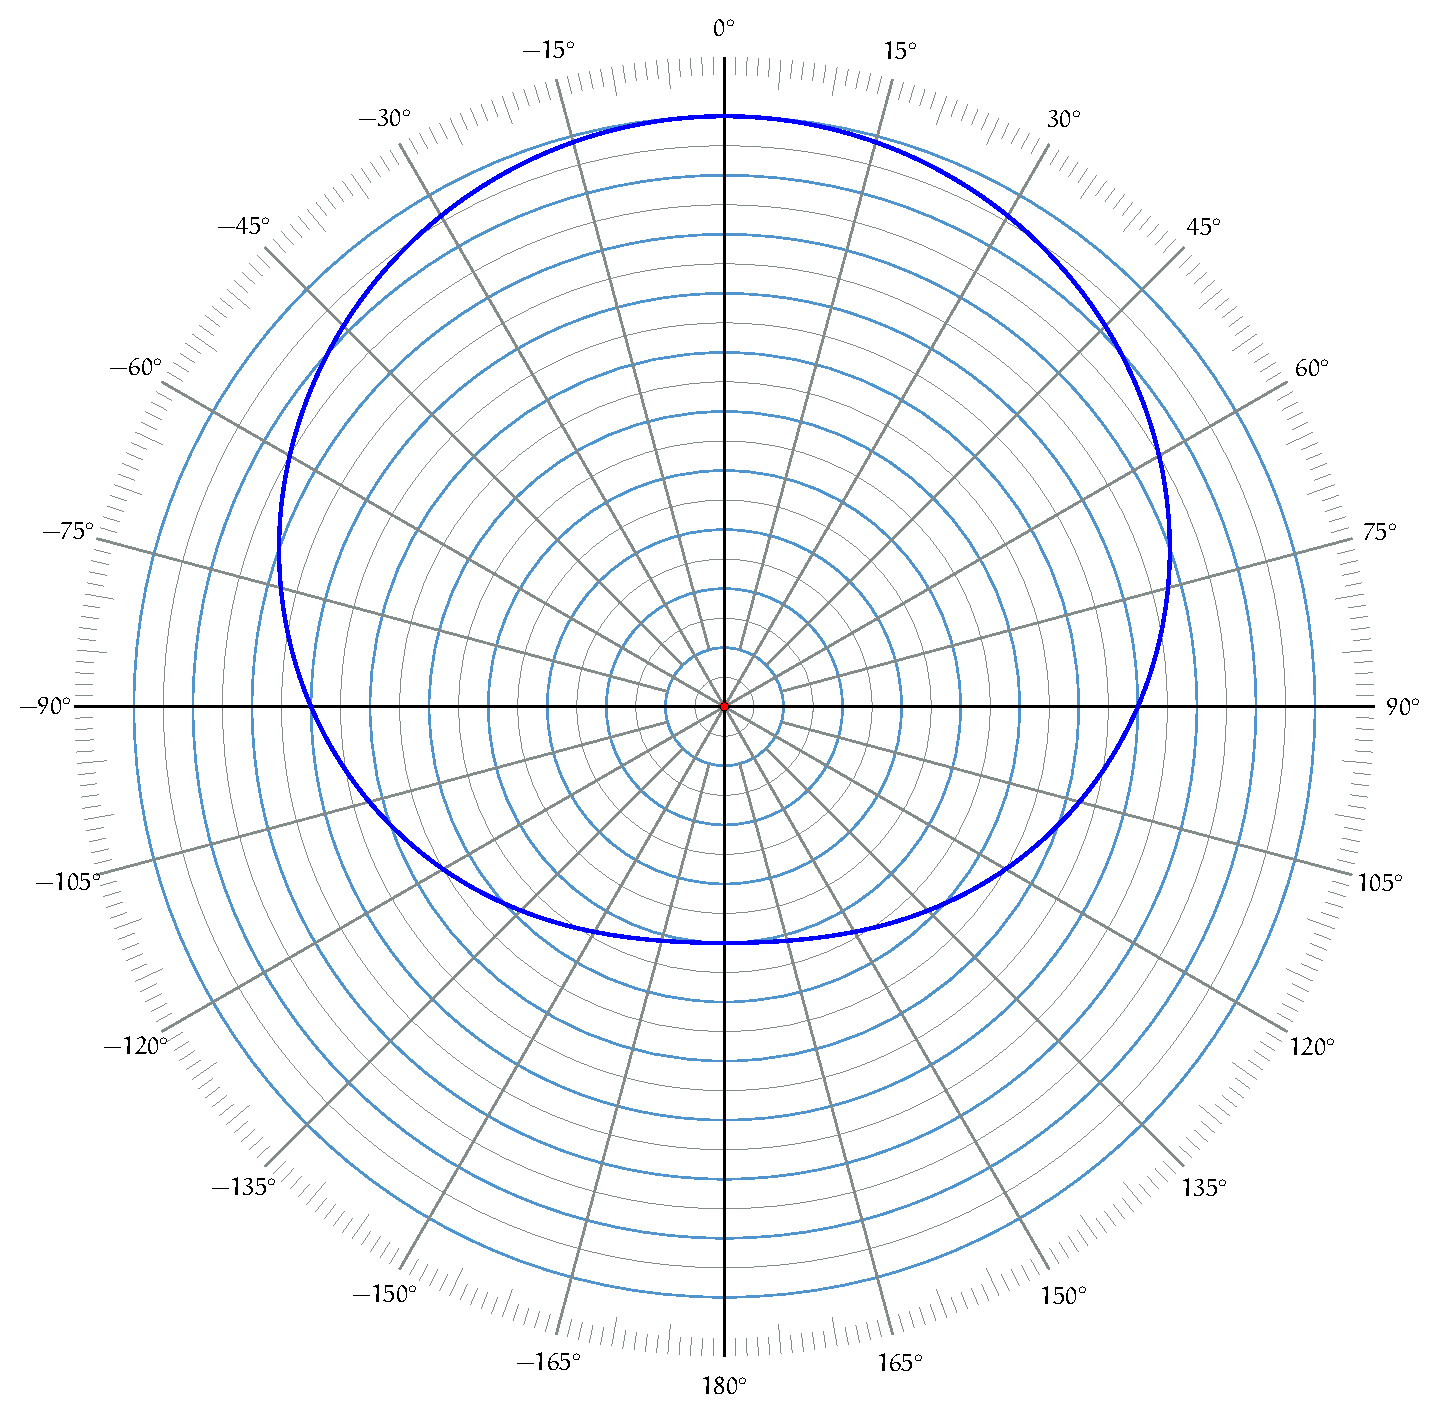
\includegraphics[height=4cm]{CAPITOLI/_TIKZ/POLAR/subcardioid}
        \caption{subcardioide. \\ Eq: $0.75(x)+0.25(x\cos\theta)$}
        \label{pol:sub-p}
    \end{subfigure}
    ~
    \begin{subfigure}[t]{0.3\textwidth}
        \centering
        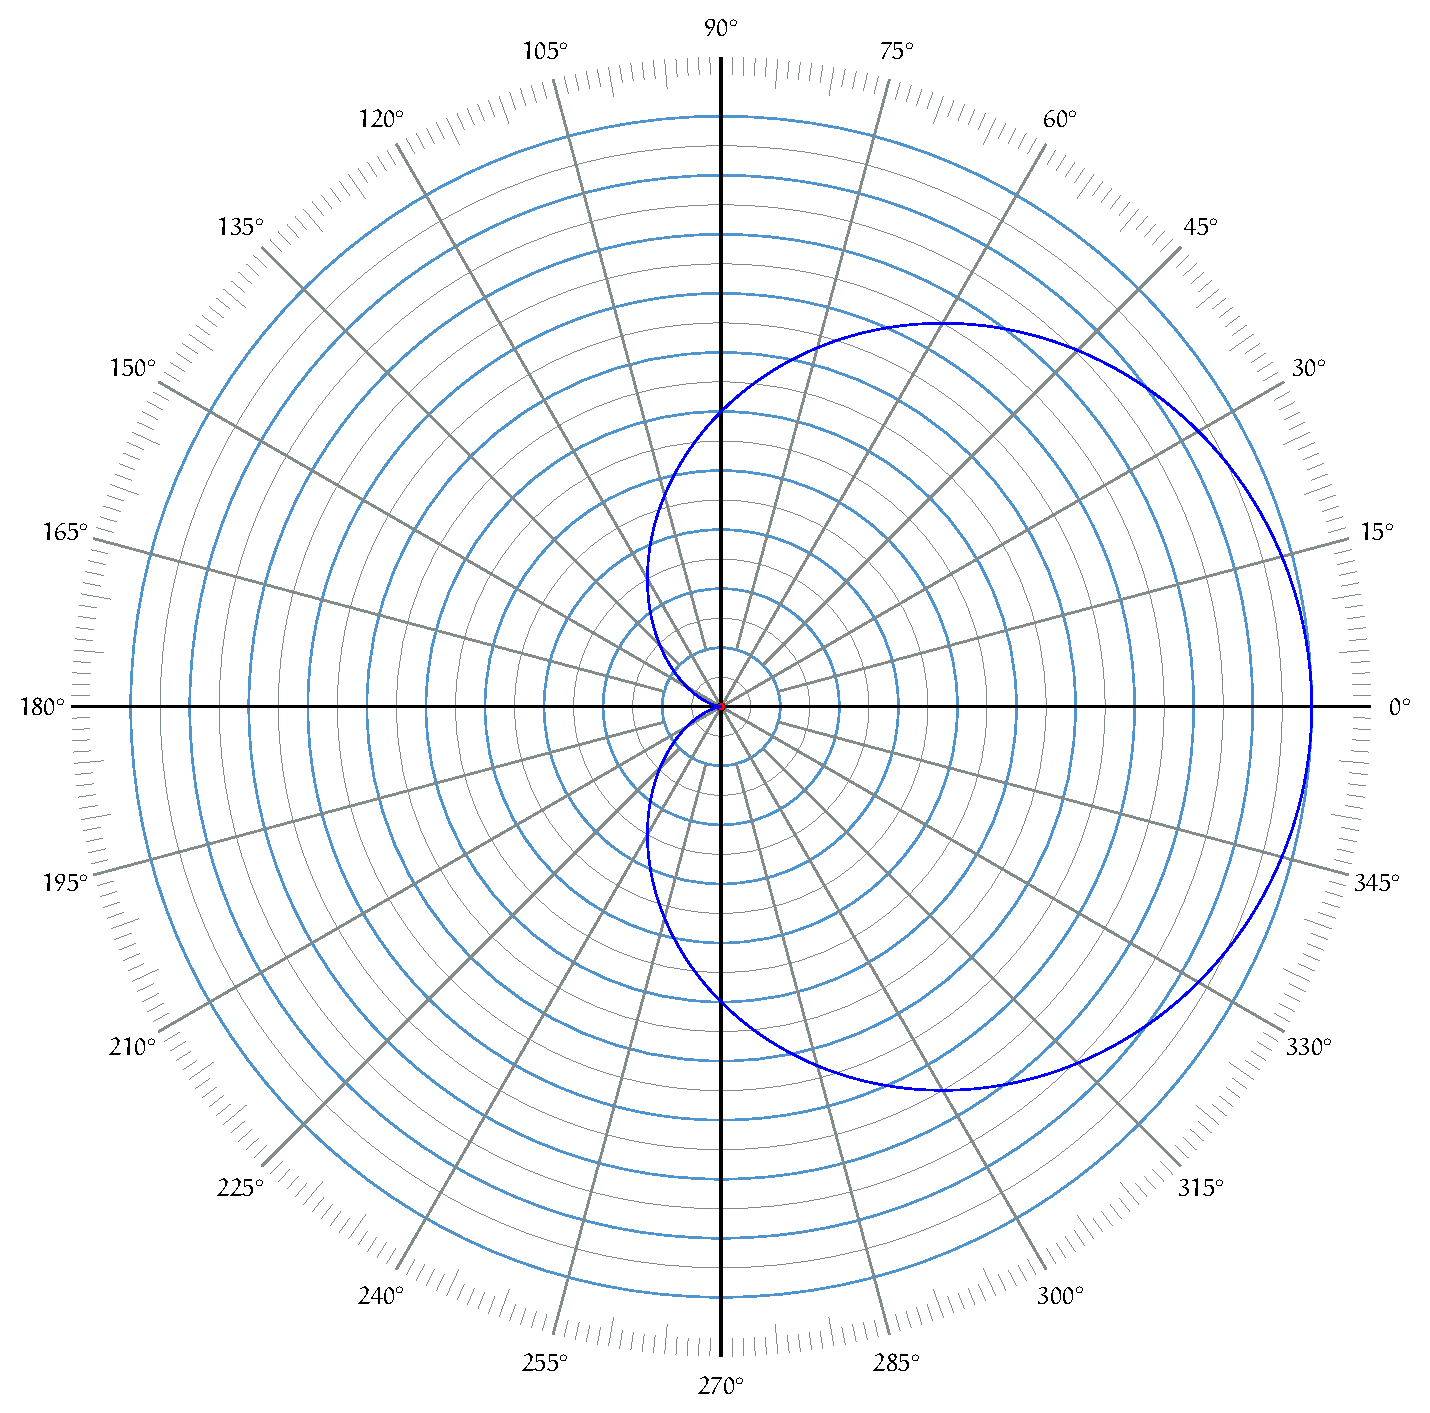
\includegraphics[height=4cm]{CAPITOLI/_TIKZ/POLAR/cardioid}
        \caption{cardioide. \\ Eq: $0.5(x)+0.5(x\cos\theta)$}
        \label{pol:cardio-p}
    \end{subfigure}
    \\
    \begin{subfigure}[t]{0.3\textwidth}
        \centering
        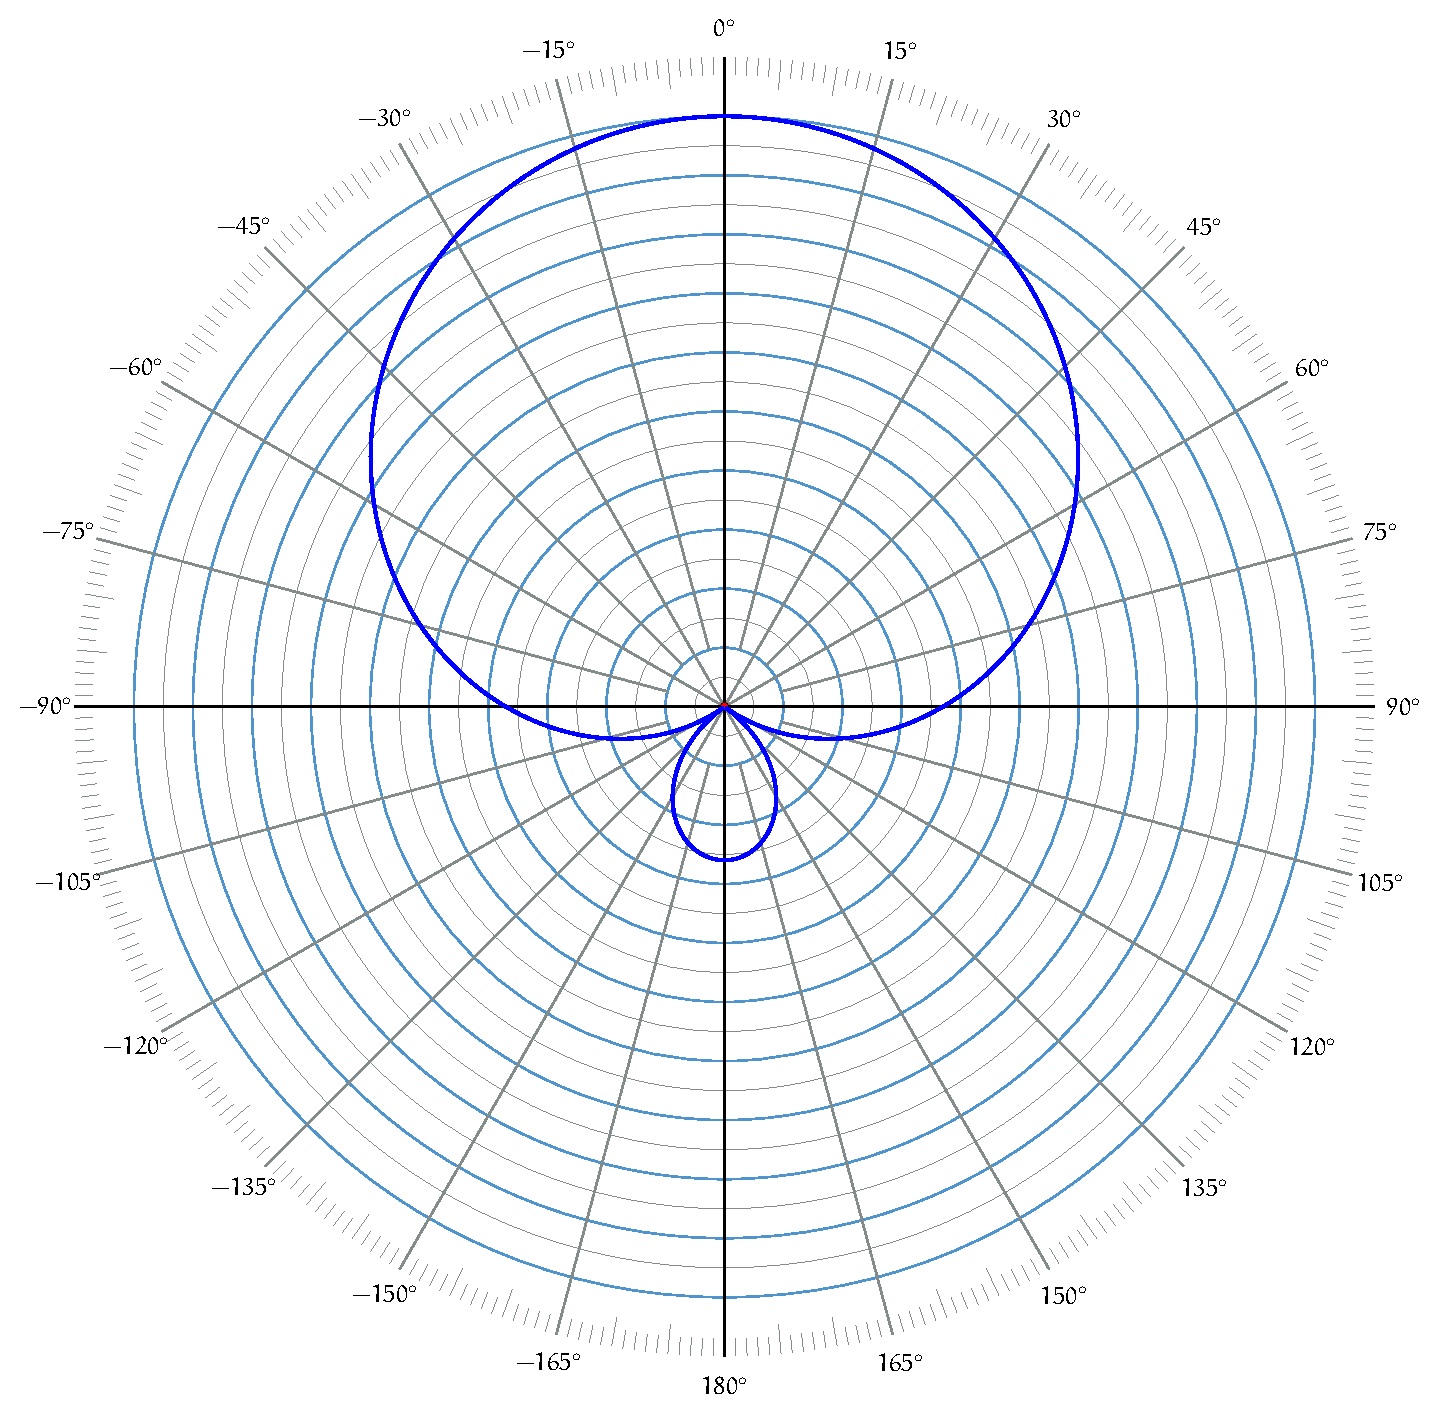
\includegraphics[height=4cm]{CAPITOLI/_TIKZ/POLAR/supercardioid}
        \caption{supercardioide. \\ Eq: $0.37(x)+0.63(x\cos\theta)$}
        \label{pol:iper-p}
    \end{subfigure}
    ~
    \begin{subfigure}[t]{0.3\textwidth}
        \centering
        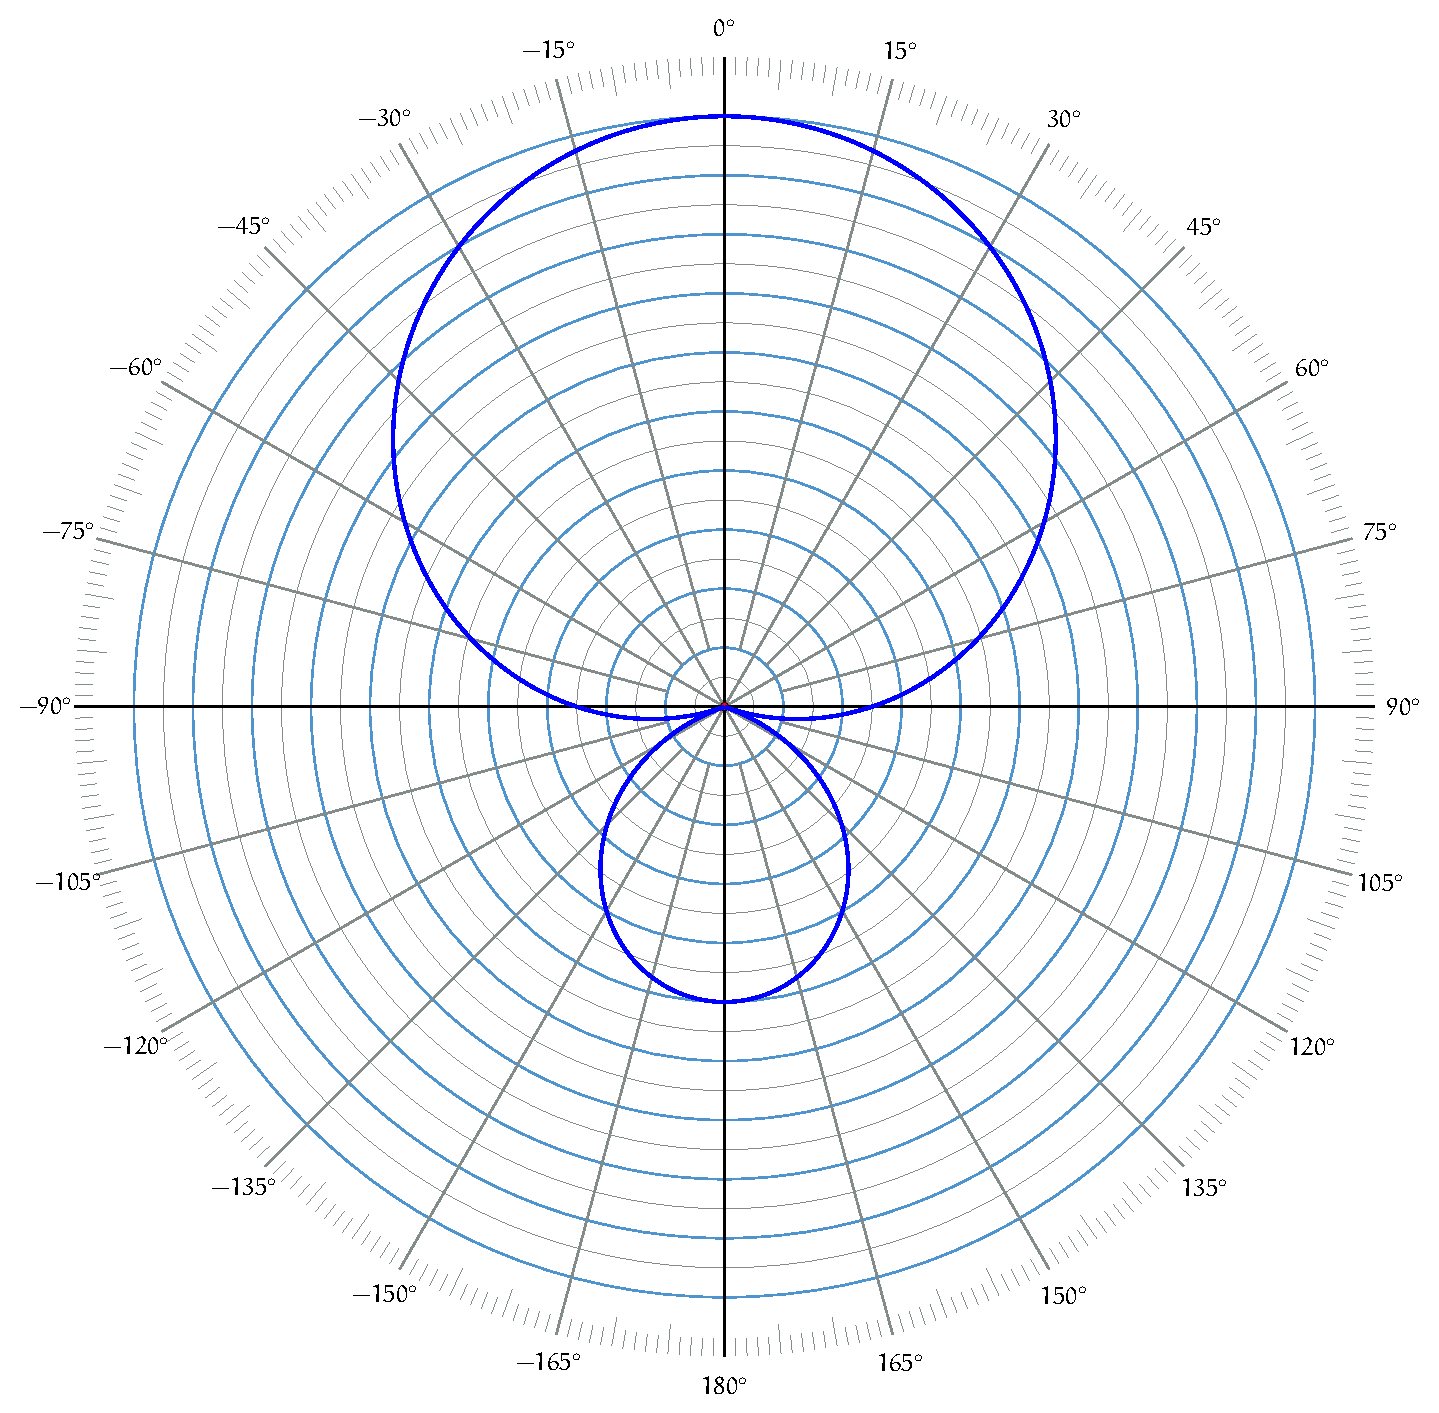
\includegraphics[height=4cm]{CAPITOLI/_TIKZ/POLAR/hypercardioid}
        \caption{ipercardioide. \\ Eq: $0.25(x)+0.75(x\cos\theta)$}
        \label{pol:iper-p}
    \end{subfigure}
    ~
    \begin{subfigure}[t]{0.3\textwidth}
        \centering
        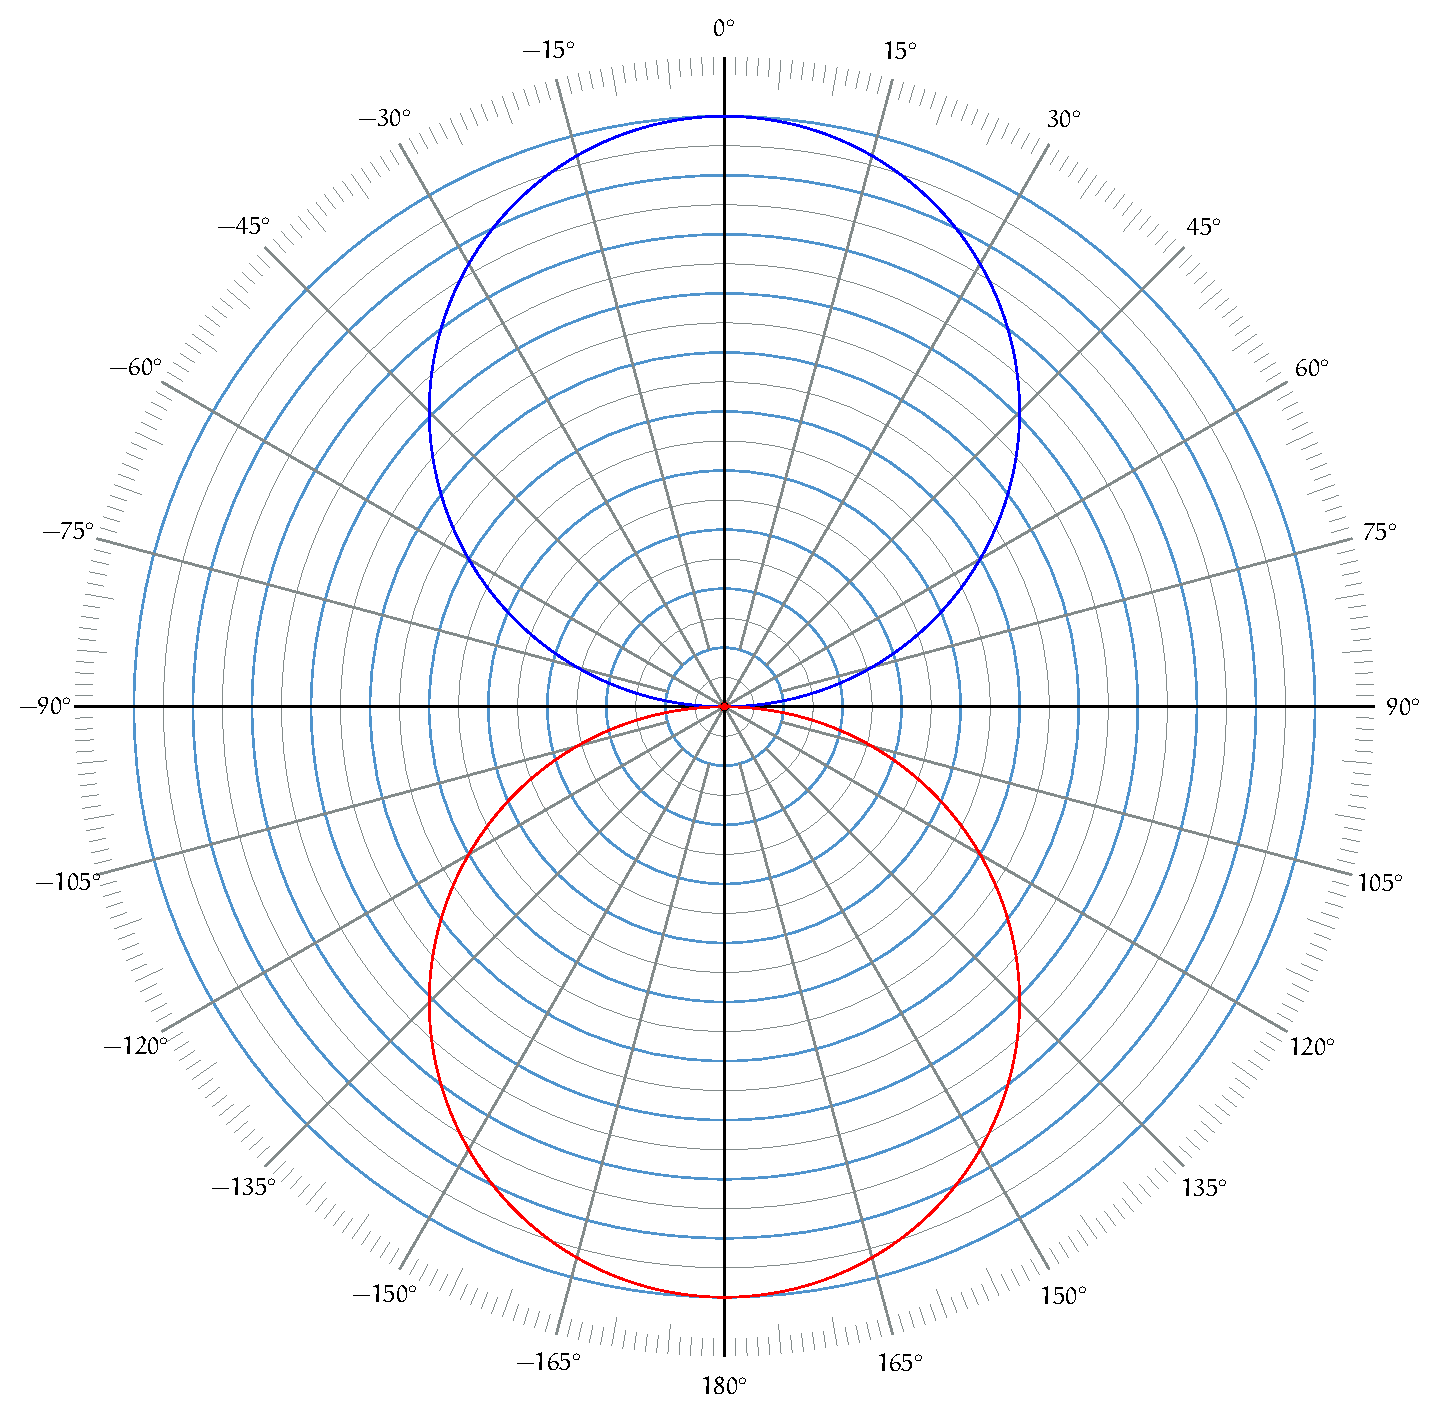
\includegraphics[height=4cm]{CAPITOLI/_TIKZ/POLAR/fig8}
        \caption{figura-8. \\ Eq: $1(x\cos\theta)$}
        \label{pol:fig8-p}
    \end{subfigure}
    \caption{Le principali figure polari ottenute mediante la calibrazione dei
    coefficienti di ampiezza della componente non-direzionale (fig. \ref{pol:omni-p}) e
    e bidirezionale (fig.\ref{pol:fig8-p}).}
    \label{pol:princicpali}
\end{figure*}
